\documentclass{beamer}

%\useoutertheme[glossy]{wuerzburg}
\useinnertheme[shadow,outline]{chamfered}
%\usecolortheme{shark}
\usecolortheme{beaver}
\beamertemplatenavigationsymbolsempty

\usefonttheme{professionalfonts}
\let\digamma\relax
\usepackage[scale=0.85,stdmathitalics=true,romanfamily=casual]{lucimatx}
\usefonttheme[stillsansseriftext]{serif}



\usepackage{fancyvrb}

%% Fancy syntax coloring via pygments
\usepackage{minted}
\definecolor{bg}{rgb}{0.95,0.95,0.95}
\usemintedstyle{borland}


\newenvironment{Rcode}
{\VerbatimEnvironment
 \begin{minted}[fontsize=\scriptsize,baselinestretch=1]{r}}%
{\end{minted}}

\newenvironment{Pcode}
{\VerbatimEnvironment
 \begin{minted}[fontsize=\scriptsize,baselinestretch=1]{python}}%
{\end{minted}}

\newenvironment{Code}[1]
{\VerbatimEnvironment
 \begin{minted}[fontsize=\scriptsize,baselinestretch=1]{#1}}%
{\end{minted}}


\usepackage{textfit} % commands \scaletoheight{height}{text} and \scaletowidth{width}{text}

\usepackage{tikz}

\usepackage{tcolorbox}

\newtheorem{Alert}{Alert}
\newtheorem{Highlight}{Highlight}

\newcommand{\Species}[1]{{\rmfamily \itshape #1}}
\newcommand{\Real}{\ensuremath{\mathbb{R}}}
\newcommand{\RealN}{\ensuremath{\mathbb{R}^n}}
\newcommand{\RealP}{\ensuremath{\mathbb{R}^p}}
\newcommand{\Mtx}[1]{\ensuremath{\mathbf{#1}}}
\newcommand{\Inv}[1]{\ensuremath{#1^{-1}}}
\newcommand{\InvMtx}[1]{\ensuremath{\mathbf{#1}^{-1}}}
\newcommand{\Red}[1]{\textcolor{red}{#1}}
\newcommand{\PsInv}[1]{\ensuremath{\mathbf{#1}^{+}}}

\usepackage{booktabs}



% --- Macro \xvec
% From a tex.stackexchange.com answer by Todd Lehman
% http://tex.stackexchange.com/questions/44017/dot-notation-for-derivative-of-a-vector
\makeatletter
\newlength\xvec@height%
\newlength\xvec@depth%
\newlength\xvec@width%
\newcommand{\xvec}[2][]{%
  \ifmmode%
    \settoheight{\xvec@height}{$#2$}%
    \settodepth{\xvec@depth}{$#2$}%
    \settowidth{\xvec@width}{$#2$}%
  \else%
    \settoheight{\xvec@height}{#2}%
    \settodepth{\xvec@depth}{#2}%
    \settowidth{\xvec@width}{#2}%
  \fi%
  \def\xvec@arg{#1}%
  \def\xvec@dd{:}%
  \def\xvec@d{.}%
  \raisebox{.2ex}{\raisebox{\xvec@height}{\rlap{%
    \kern.05em%  (Because left edge of drawing is at .05em)
    \begin{tikzpicture}[scale=1]
    \pgfsetroundcap
    \draw (.05em,0)--(\xvec@width-.05em,0);
    \draw (\xvec@width-.05em,0)--(\xvec@width-.15em, .075em);
    \draw (\xvec@width-.05em,0)--(\xvec@width-.15em,-.075em);
    \ifx\xvec@arg\xvec@d%
      \fill(\xvec@width*.45,.5ex) circle (.5pt);%
    \else\ifx\xvec@arg\xvec@dd%
      \fill(\xvec@width*.30,.5ex) circle (.5pt);%
      \fill(\xvec@width*.65,.5ex) circle (.5pt);%
    \fi\fi%
    \end{tikzpicture}%
  }}}%
  #2%
}
\makeatother

% --- Override \vec with an invocation of \xvec.
\let\stdvec\vec
\renewcommand{\vec}[1]{\xvec[]{#1}}
% --- Define \dvec and \ddvec for dotted and double-dotted vectors.
\newcommand{\dvec}[1]{\xvec[.]{#1}}
\newcommand{\ddvec}[1]{\xvec[:]{#1}}


\usepackage{pifont}
\newcommand{\weblink}{\ding{43}}  % hand with pointing finger

\definecolor{links}{HTML}{2A1B81}
\hypersetup{colorlinks,linkcolor=,urlcolor=magenta}

\usepackage{pdfpages}

\parskip=0.5em

%===========================================================
\title{Scientific Computing for Biologists}
\subtitle{Lecture 9: (Dis)similarity and clustering}

\author{Instructor: Paul M. Magwene}
\date{30 October 2012}


\begin{document}

\begin{frame}
\titlepage
\end{frame}



%===========================================================
\begin{frame}
  \frametitle{Outline of Lecture}
  
\begin{itemize}
    \item Distance and dissimilarity measures
    \begin{itemize}
        \item Quantitative data
        \item Dichotomous data
        \item Qualitative data
    \end{itemize}
    \item Hierarchical clustering
    \item Neighbor-joining
    \item Minimum Spanning Tree (MST)
    \item K-means clustering
\end{itemize}     
  
\end{frame}
%===========================================================

%===========================================================
\begin{frame}
  \frametitle{Similarity/Dissimilarity}

\begin{block}{Intuition}
Similarity is a measure of ``likeness'' between two entities of interest. Dissimilarity is the complement of similarity.
\end{block}


\begin{itemize}
\item Dissimilarities may be converted to similarities (and vise versa) by taking any monotonically decreasing function. For example:
\[
s = 1 - d_{ij}  \ \mbox{(for $0 \leq d_{ij} \leq 1$)}
\]
\item Dissimilarities are usually in range $0 \leq d_{ij} \leq C$ where $C$ is the maximum dissimilarity
\item Distances are one measure of dissimilarity but distances are unbounded to the right
\[
d_{ij} \in [0,\infty]
\]
\end{itemize}
\end{frame}
%===========================================================

%===========================================================
{ 
\setbeamercolor{background canvas}{bg=} 
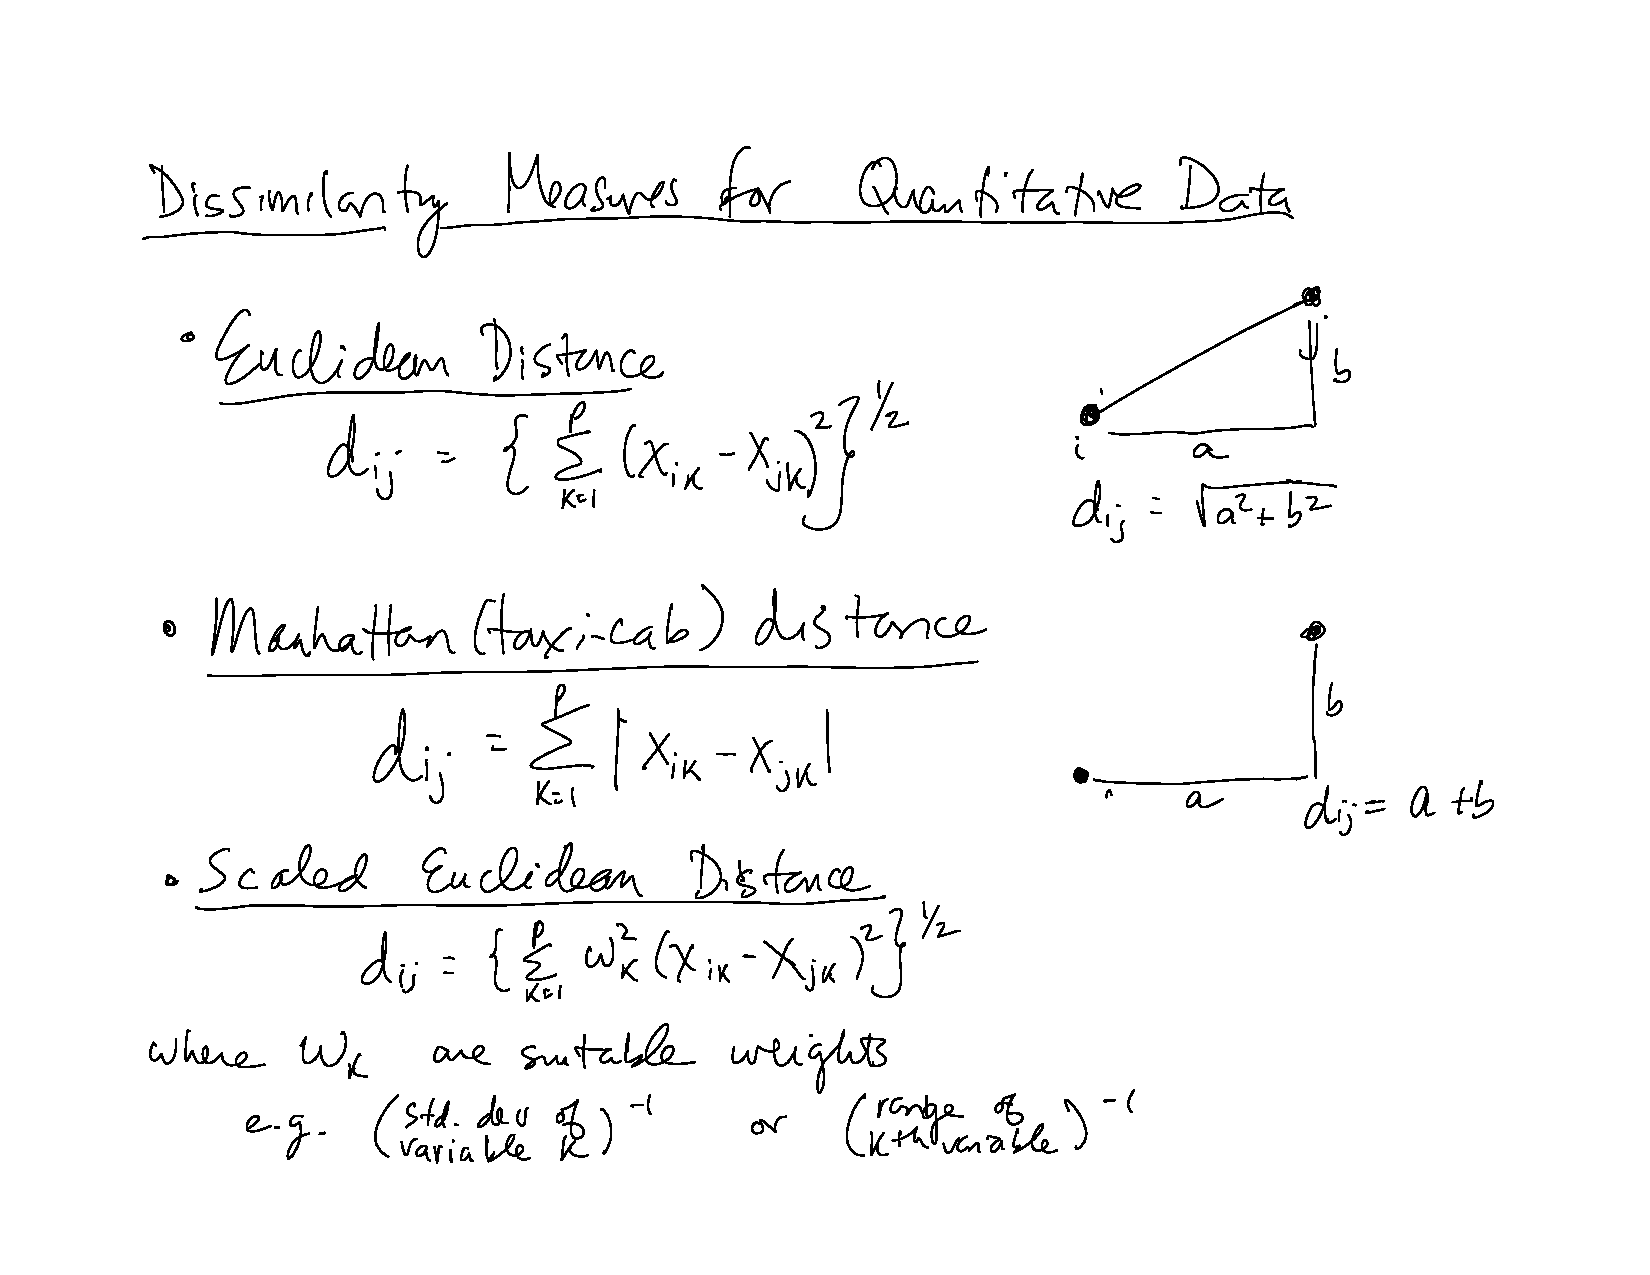
\includepdf[pages={1-5,8-16}]{lecture7-clustering.pdf}
}
%===========================================================

%===========================================================
%% Neighbor-joining

\begin{frame}[shrink=5]
\frametitle{Neighbor Joining}

Originally described by Saitou and Nei, 1987.

\begin{block}{Goal}
Tries to create the (unrooted) tree topology with the least branch length
(minimum-evolution criterion).
\end{block}

Basic algorithm:
\begin{enumerate}
\item Calculate matrix $Q$ (next slide) from the distance matrix
\item Find the pair of taxa in $Q$ with the lowest value; create a node on the tree that joins these two taxa (i.e. the closest neighbors)
\item Calculate the distance of each of the taxa in the pair to this new node
\item Calculate the distance of all taxa outside of this pair to the new node
\item Repeat from step 1 using the distances calculated in the previous step
\end{enumerate}

\end{frame}
%===========================================================

%===========================================================
\begin{frame}
\frametitle{Neighbor Joining, cont.}

\[
Q_{ij} = (r - 2) d_{ij} - (R_i + R_j)
\]

where $r$ is the number of taxa, $d_{ij}$ is the distance between taxa $i$ and $j$ and $R_k$ is the row sum over row $k$ of the distance matrix ($R_k=\sum_i d_{ik}$).

\medskip

When nodes $i$ and $j$ are joined they are replaced by a node, $A$, with distance to a remaining node $k$ given by:
\[
d_{Ak} = \frac{1}{2} (d_{ik} + d_{jk} - d_{ij})
\]
    
\end{frame}
%===========================================================

%===========================================================
\begin{frame}
\frametitle{NJ example from Saitou and Nei 1987}
\begin{center}
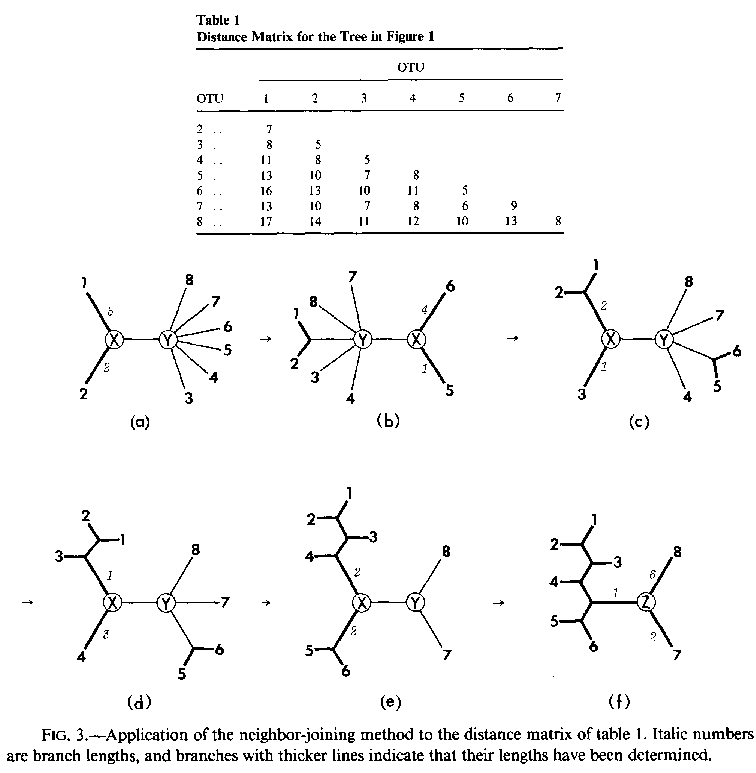
\includegraphics[height=3.2in]{saitou-nj-example.pdf}    
\end{center}
\end{frame}
%===========================================================




%===========================================================
\begin{frame}
  \frametitle{Minimum Spanning Tree}

\begin{block}{Goal}
Construct a tree that connects all points in the data set and whose total length is minimized.
\end{block}

\emph{Statistical applications}
\begin{itemize}
    \item highlights close neighbors in a data set
    \item useful check for distortions produced by projection techniques
    \item tests of normality
\end{itemize}
\medskip

\emph{Other applications}
\begin{itemize}
    \item urban planning/engineering
    \item circuit design
\end{itemize}

\end{frame}
%===========================================================

%===========================================================
\begin{frame}
  \frametitle{Example Data Set}

\begin{center}
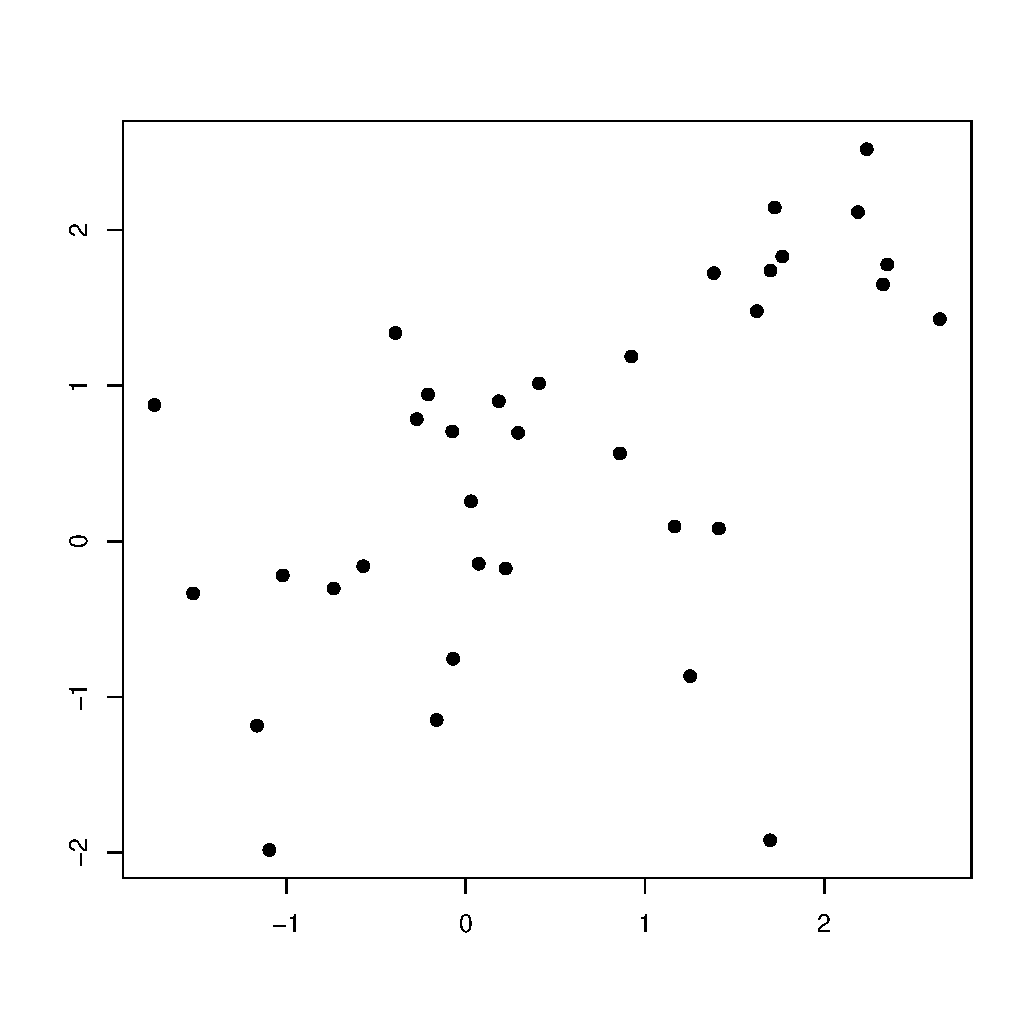
\includegraphics[height=3.1in]{points-only}
\end{center}
\end{frame}
%===========================================================

%===========================================================
\begin{frame}
  \frametitle{Minimum Spanning Tree: Example}

  
\begin{center}
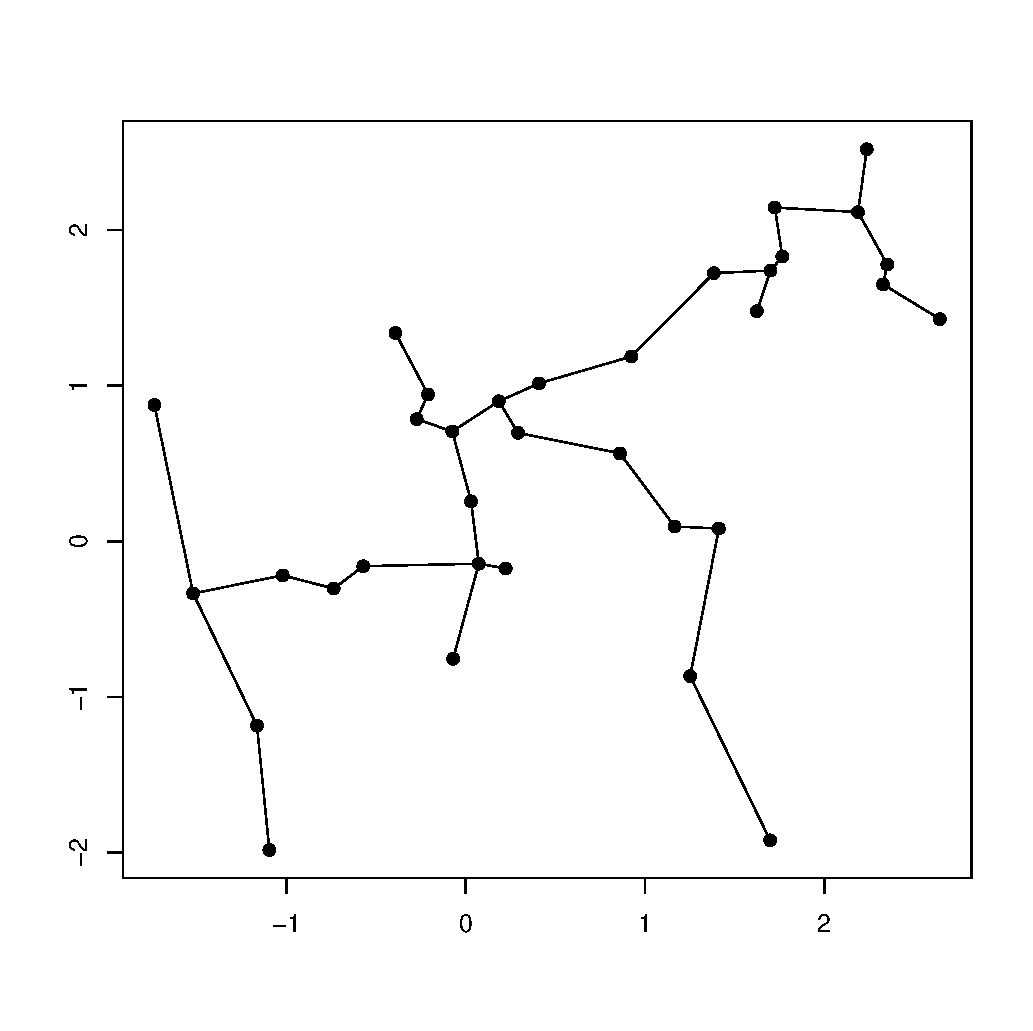
\includegraphics[height=3.1in]{points-mst}
\end{center}
\end{frame}
%===========================================================

%===========================================================
\begin{frame}
  \frametitle{Relationship between MST and Single Linkage Clustering}


\begin{itemize}

\item Cut a single linkage dendrogram at height, $\delta \dashrightarrow$ clusters

\item Remove all edges in the MST with length $\geq \delta \dashrightarrow$ subgraphs corresponding to the same clusters

\end{itemize}

\end{frame}
%===========================================================

%===========================================================
\begin{frame}
  \frametitle{A Generic MST Algorithm}


\textbf{Input}: dissimilarity matrix, \Mtx{D}, between each object (point) of interest
\begin{enumerate}
\item Create a graph, G, where  $V = \{v_1,\ldots,v_n\}$ and $E =\{\}$ ($E$ initially empty)
\item Find the smallest dissimilarity, $d_{ij}$ where (i,j) is not in $E$.
\item Add (i,j) to $E$ if (i,j) does not create a cycle
\item Repeat from step 2 until every vertex is included in at least one edge
\end{enumerate}

Not particularly efficient algorithm, but simple. More efficient algorithms for finding MSTs include Kruskal's Algorithm and Prim's algorithm.

\end{frame}
%===========================================================

%===========================================================
\begin{frame}
  \frametitle{Applications of the MST}

MST tends to highlight close neighbors; can be used to look for distortions associated with projections to lower dimensional spaces.

\begin{block}{Using the MST to look for Projection Distortion}
\begin{itemize}
    \item  Calculate the MST based on dissimilarity in a high-dimensional space
    \item Draw the MST edges among points in the projection space (e.g. MDS or PCA)
    \item MST edges that cross highlight geometric relationships among points that are not well represented by the projection
\end{itemize}
\end{block}
\end{frame}
%===========================================================

%===========================================================
%% K-means clustering

\begin{frame}
\frametitle{K-mean Clustering}

\begin{block}{General idea}
Assign the $n$ data points (or $p$ variables) to one of $K$ clusters to as to optimize some criterion of interest.    
\end{block}

\begin{columns}
    
\begin{column}{5cm}
\begin{itemize}
\item The most common criterion to minimize is the sum-of-squares from the group centroids.

\[
V = \sum_{i=1}^k \sum_{j \in g_i}|x_j-\mu_i|^2
\]
\end{itemize}
\end{column}

\begin{column}{5.5cm}
\begin{center}
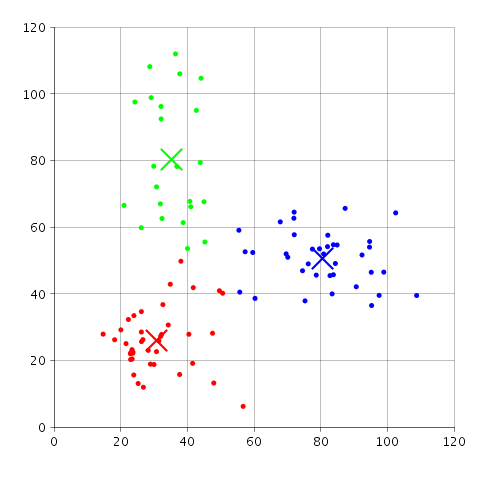
\includegraphics[width=0.9\textwidth]{k-means-simple.png}    
\end{center}
\end{column}

\end{columns}


\end{frame}
%===========================================================

%===========================================================
\begin{frame}
\frametitle{Simple algorithm for K-means clustering}
\begin{enumerate}
\item Decide on $k$, the number of groups

\item Randomly pick $k$ of the objects to act as the initial centers

\item Assign each object to the group whose center it is closest to

\item Recalculate the $k$ centers as the centroids of the objects assigned to them

\item Repeat from step 3 until centroids no longer move (convergence)

\end{enumerate}
\end{frame}
%===========================================================

%===========================================================
\begin{frame}
\frametitle{Illustration of K-means algorithm}
\begin{center}
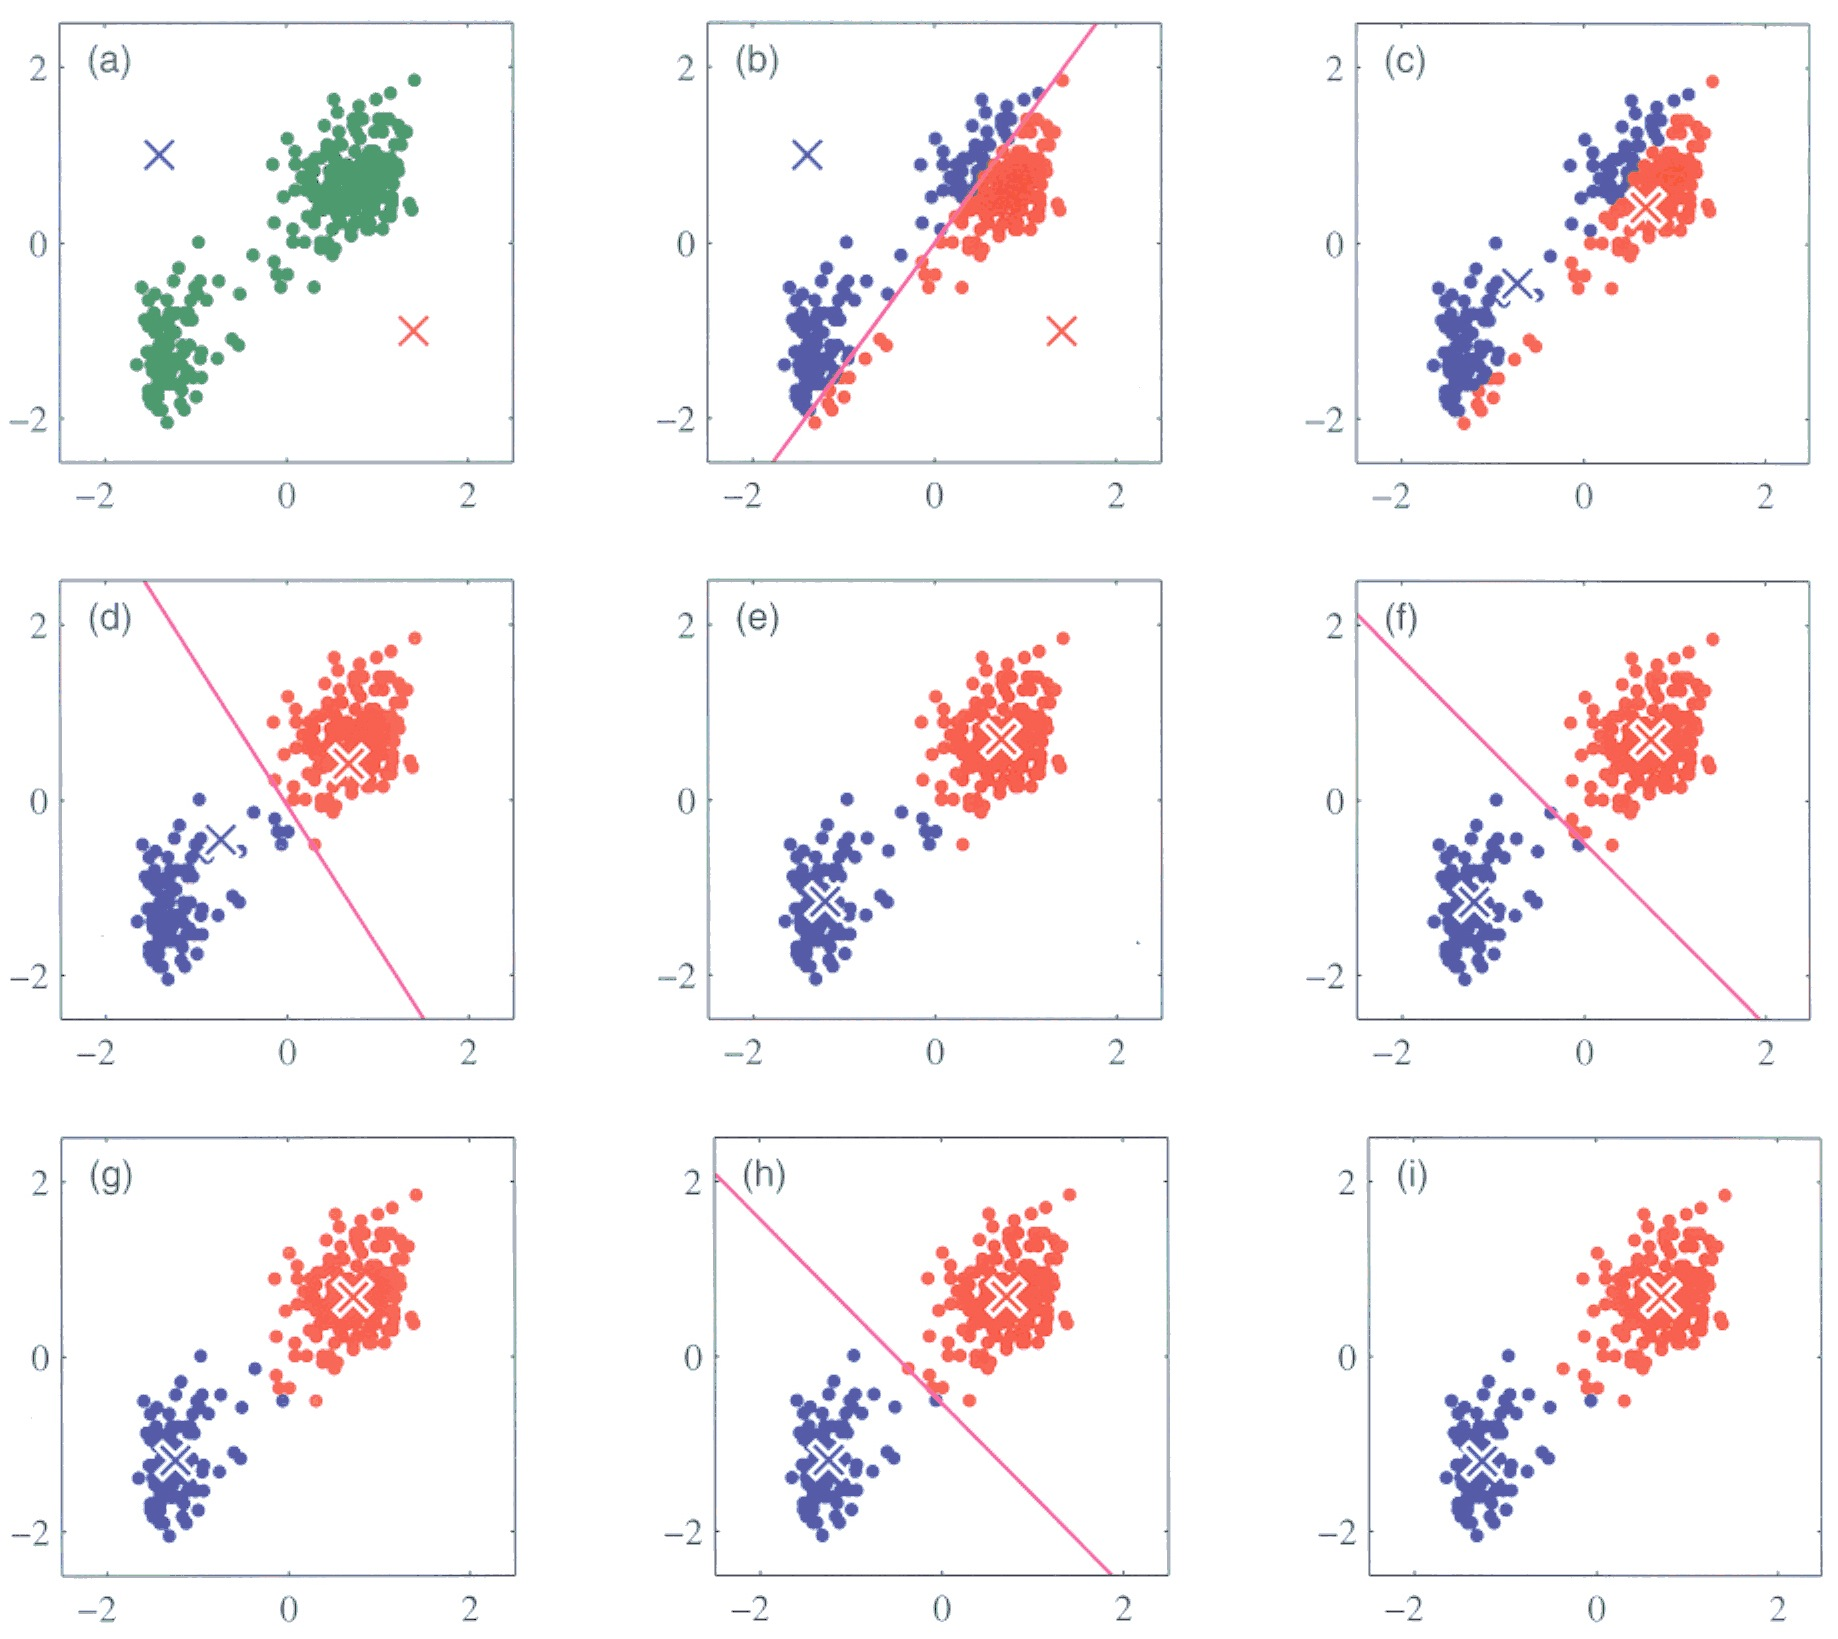
\includegraphics[height=3.2in]{k-means-fig.jpg}    
\end{center}
\end{frame}
%===========================================================

%===========================================================
\begin{frame}
\frametitle{Things to note re:K-means clustering}
\begin{itemize}
\item The algorithm described above does not necessarily find the global optimum

\bigskip

\item The algorithm is sensitive to choice of initial cluster center; k-means is often run multiple-time with different initial centers to insure inferred clusters are robust.    
\end{itemize}
\end{frame}
%===========================================================



\end{document}



%===========================================================
\begin{frame}
  \frametitle{XXX}

\end{frame}
%===========================================================

